\section{Heavy flavour production and spectroscopy }


%\subsection{Introduction and motivation}

Quantum Chromodynamics (QCD), and the quark model out of which it grew, 
is one of the fundamental building blocks of the SM.
It has been extensively validated over the decades, and is
very well understood. However, due to the non-perturbative behaviour
that follows from the large self-coupling of low-energy gluons,
the practical implications of QCD are still
very much an active subject of research. This was vividly illustrated
in the realm of spectroscopy recently, when the first compelling
observation of pentaquark ($qqqq\bar{q}$) states was made by LHCb~\cite{Aaij:2015tga}
just over fifty years after their existence was predicted~\cite{GellMann:1964nj}.
This discovery, illustrated in figure~\ref{figspect} left, came as a surprise to experimentalists and theorists alike:
the possible existence of such states was known, but the quark composition of
quasi-stable pentaquark resonances (let alone their masses, widths, and
production mechanisms) was not.

More broadly, results from QCD and strong physics are frequently
needed as inputs to other measurements or to their interpretation.
For example, there is considerable interest in the decays
$\Bbar \to D^{(*)} \lepton^- \neulb$: the ratio of branching fractions
(in a restricted region of phase space) for $\lepton=\muon$ and $\lepton=\tauon$
can be used to test lepton universality. The current world average,
combining results from LHCb, BaBar and Belle, is in tension
at the $4\sigma$ level with SM expectations~\cite{bib:hfag}.
One of the important systematic uncertainties in this measurement
is associated with the spectrum and properties of excited charm resonances $D^{**}$,
which could contaminate the final state with feed-down from
$\Bbar \to D^{**} \lepton^- \neulb$: here, input from spectroscopy is
needed for the measurement itself. There are numerous instances
in which QCD input is needed for the interpretation of measurements,
notably for $\Bz \to \Kstarz \mup \mun$ in which 
an overall tension of $3.4\sigma$ with the SM prediction of~\cite{Descotes-Genon:2014uoa} has been seen. 
The significance of this 
tension depends strongly upon the SM theory prediction and its
uncertainties. To take a third and final example, QCD processes are
an inherent background to all physics at the LHC, and in some cases
Monte Carlo predictions of their spectrum need to be included in the
fit itself. Tuning of the Monte Carlo models requires not only work
from the phenomenology community but also measurements of production
cross-sections across a range of transverse momentum and
pseudorapidity.

%\subsection{(Past and current work in the French community)}


\begin{figure}[h]
\begin{center}
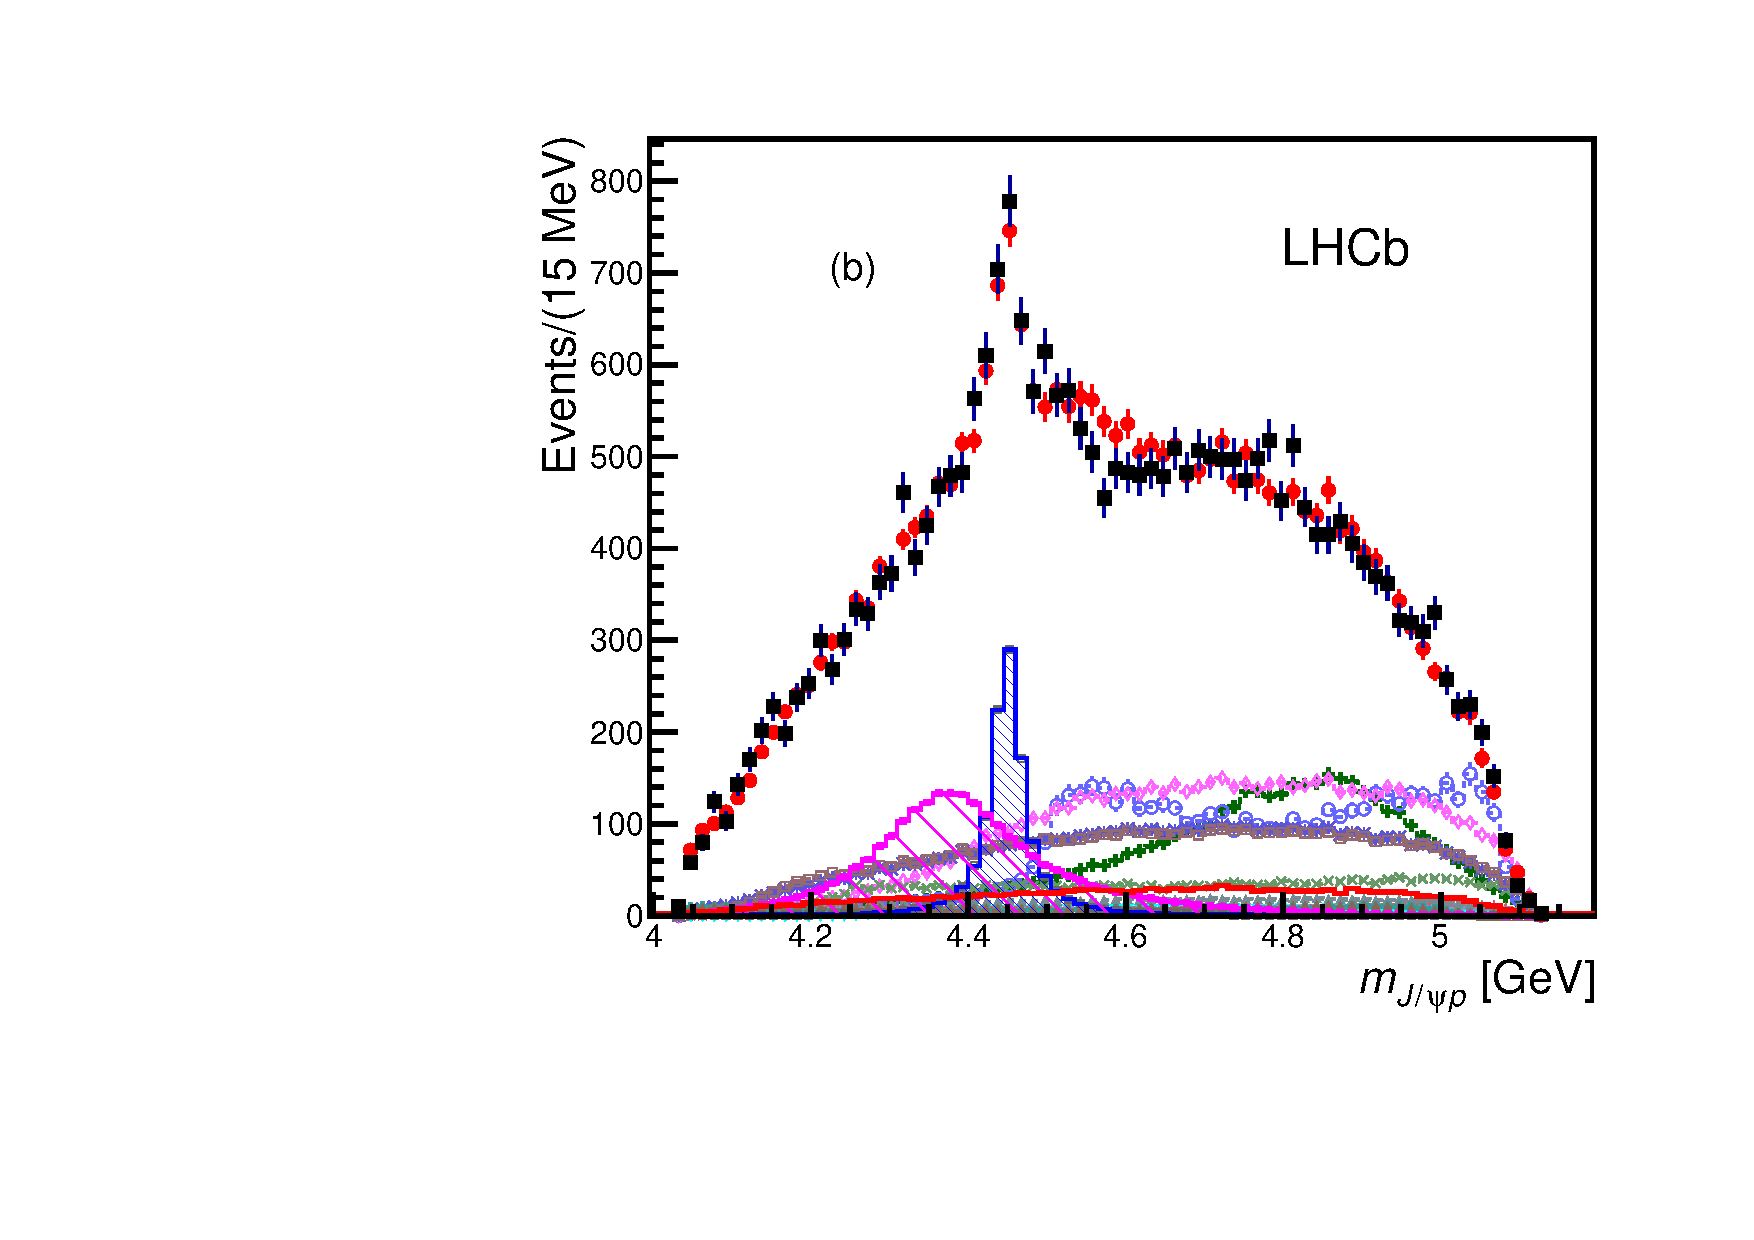
\includegraphics[width=6.5cm]{mjpsip-default.pdf} 
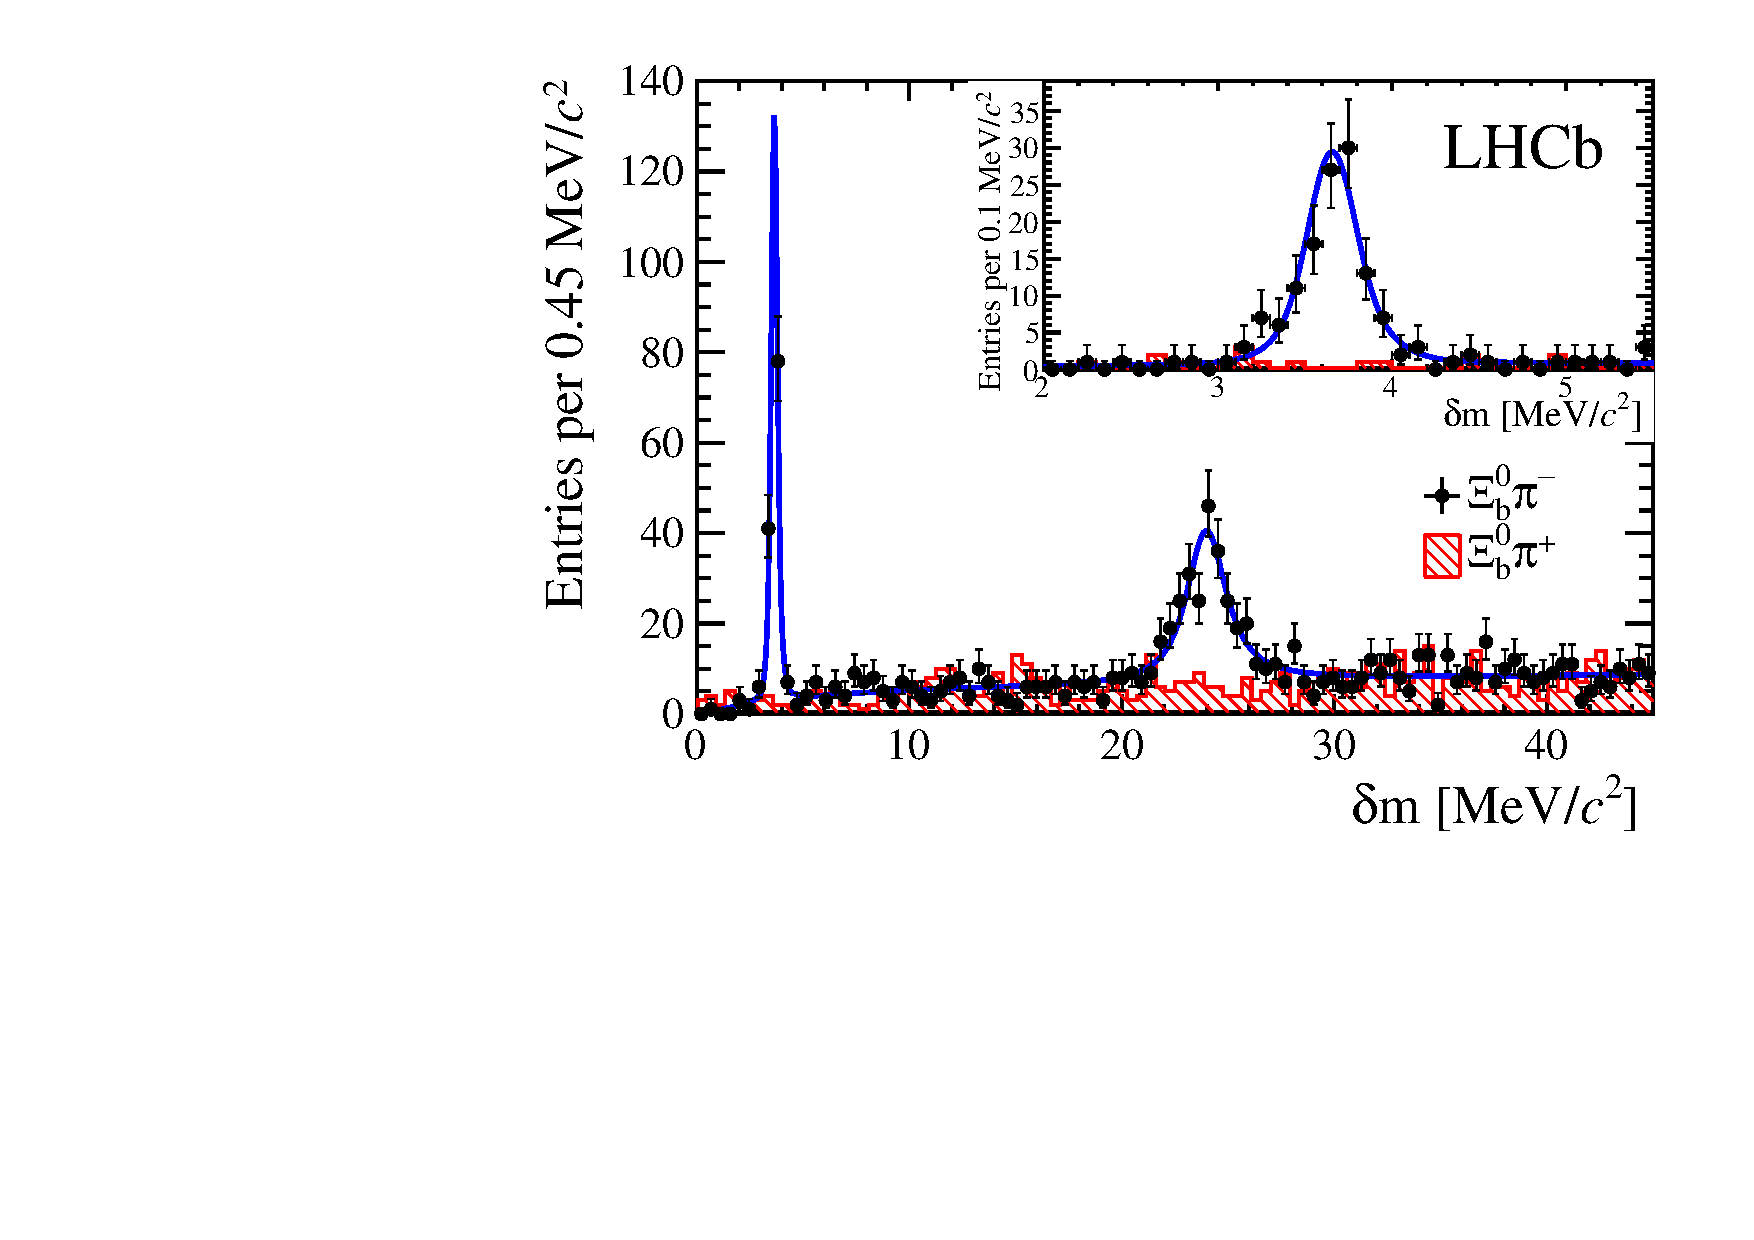
\includegraphics[width=7.5cm]{paperPlot-merged.pdf}
\end{center}
\caption{Left plot: results of a fit to $\Lb \to \jpsi \Km \proton$ decays in the Run1 LHCb data. The figure is taken from Ref.~\cite{Aaij:2015tga}, which reported the first observation of these two pentaquark states, the $P_c(4380)^+$ and $P_c(4450)^+$. Their amplitudes are shown as hatched magenta and blue histograms.  Right plot: results of a fit to the $\Xibz \pim$ spectrum in the Run1 LHCb data. The figure is taken from Ref.~\cite{Aaij:2014yka}, which reported the first observation of these two resonances, the \XibPrimeMinus and \XibStarMinus. The inset shows a zoom around the first peak.}%
\label{figspect}%
\end{figure}




The HEP community in France is engaged in this field, both on
the experimental and theory sides. For practical reasons most
experimental measurements have come from LHCb in recent years.
LHCb-France has been involved on multiple fronts:
spectroscopy of exotica,  %(LAL, LAPP, LPNHE),
spectroscopy of non-exotic resonances %(LAL, LPNHE),
and measurements of production rates.  %(CPPM, LAL, LAPP, LPNHE).
This list is not exhaustive, and there are far too many
results to discuss them individually; purely by way of
illustration we point to recent contributions by French groups to 
%
studies of exotic 4- and 5-quark resonances~\cite{Aaij:2016ymb, Aaij:2014jqa}, 
%
discoveries of two $\Xi_b$ resonances and precise measurements
of their mass splittings~\cite{Aaij:2016jnn, Aaij:2014yka} (illustrated in figure~\ref{figspect} right), 
%
and measurements of the $J/\psi$ production cross-section
with the new 13\,TeV LHC data~\cite{Aaij:2015rla}.
Numerous theory groups are also actively involved, and
we do not dare attempt an exhaustive list. %\footnote{  In the author list of one review paper of heavy flavour  production alone [\cite{Andronic:2015wma}],  we counted eight French laboratories:  IPNO, IRFU, LAL, LAPTh, LLR, LPC, LPSC, and SUBATECH.}.
As well as hadron production, there is substantial French
expertise in spectroscopy theory. 

%THIS GUY IS NOT IN THE GDR AT THE MOMENT SO I WOULD NOT INCLUDE THIS 
%For example, the opening
%theory review talk at the 
%2014 Workshop on Heavy Quark Baryons at LHCb\footnote{
%  \url{https://indico.cern.ch/event/317758/}
%}, a workshop organized by LHCb to which external experts were invited,
%was given by a member of IPNL. This is both recognition of
%this expertise and an illustration of the demand for
%productive exchanges between theory and experiments.


% Note that IPNL = IPN Lyon (vs IPN at Orsay)
%
% IPNL includes Jean-Marc Richard, an expert on hadron spectroscopy

% Note especially : arXiv:1407.8526

%\subsection{(proposed work in the 4 coming years)}




\subsection*{Plans for the GDR}
During the coming years, several analyses in this area are
planned by members of LHCb in France and will be followed in the framework of the GDR.  
By way of example, these include:
%
\begin{itemize}
\item Studies in beauty baryon spectroscopy following on from the observations
of three $\Xi_b$ resonances;
\item Searches for the doubly heavy
$\Xi_{cc}$ baryons;
\item Measurements of production cross-sections
at new centre-of-mass energies (including the 13\,TeV Run2
data and in heavy-ion collisions).
\end{itemize}

Assuming that the $\Xi_{cc}$
searches are successful, they in particular will lead to fruitful
exchanges with theory: their masses and properties will have
immediate implications for QCD models, and theory input will be
very useful for the next step, namely observing and studying their
excitations.




